\documentclass[journal]{IEEEtran}

% Additional packages
\usepackage{graphicx}
\usepackage{amsmath}
\usepackage{lipsum}
\usepackage{url}
\begin{document}

\title{Elastic Collision of Two Discs with Equal Mass: Investigating Momentum and Kinetic Energy Conservation}
\author{IBRAHIM H.I. ABUSHAWISH\\ Instructor: Arş.Gör.Dr.\\ Group ID: 4, Course \& Section Number: PHYS1203\\Experiment Date: 19 April, Report Submission Date: 6 May}

\maketitle

\begin{abstract}
This experiment explores the conservation of momentum and kinetic energy during the elastic collision of two discs of equal mass. The analysis includes the application of relevant equations and considerations for imperfect experimental conditions.
\end{abstract}

\section{Introduction}
In physics, momentum ($p = mv$) and kinetic energy ($K = \frac{1}{2} mv^2$), are fundamental concepts that play a crucial role in understanding the motion of objects, where $m$ (0.530 $kg$ for each) and $v$ are mass and velocity respectively. In ideal elastic collisions, both momentum and kinetic energy are conserved.

An elastic collision is defined as a collision in which both momentum and kinetic energy are conserved. This means that the total momentum and the total kinetic energy of the system remain constant before and after the collision.

The conservation of momentum in a collision involving two objects can be expressed as:
\begin{equation}
    p_{\text{initial}} = p_{\text{final}}
    \label{eq:momentum_con}
\end{equation}

Similarly, the conservation of kinetic energy can be expressed as:
\begin{equation}
    K_{\text{initial}} = K_{\text{final}}
    \label{eq:energy_con}
\end{equation}

However, even though elastic collisions aim for perfect conservation of momentum and kinetic energy, environmental imperfections or experimental errors can cause slight deviations in the measured values before and after the collision.


\section{Experimental Setup}
The experimental setup shown in Fig~\ref{fig:setup}:
\begin{figure}
    \centering
    
\includegraphics[width=\linewidth]{setup.jpg}
    \caption{Experimental setup with the two steel discs connected with a spark oscillator (back of the setup) and an air compressor (blue, up-right corner) over the recording paper.}
    \label{fig:setup}
\end{figure}
The experiment utilizes two discs of equal mass on a low-friction surface. To achieve that, an air compressor compresses air between the discs and the surface, ensuring an elastic collision. A paper with a spark oscillator is employed to plot trajectory points at 0.1-second intervals setting.
\newpage
\section{Procedure}
The total momentum of the system either before or after the collision is calculated from the following equations: 
\begin{equation}
    P_x = mv_acos\theta_a + mv_bcos\theta_b
    \label{eq:px}
\end{equation}
\begin{equation}
    P_y = mv_asin\theta_a + mv_bsin\theta_b
    \label{eq:py}
\end{equation}
\begin{equation}
    |\Vec{P}| = \sqrt{p_x^2 + p_y^2}
    \label{eq:ptotal}
\end{equation}

In a two-dimensional collision scenario, the equations (~\ref{eq:px}-~\ref{eq:ptotal}) provided describe the x-component and y-component of the total momentum, denoted as $P_x$ and $P_y$ respectively. Here, $m$ represents the mass of the objects involved, while $v_a$ and $v_b$ are the magnitudes of the velocities of the objects along their respective directions. The angles $\theta_a$ and $\theta_b$ represent the orientations of these velocities with respect to the x-axis. By utilizing trigonometric functions, the equations (\ref{eq:px}, \ref{eq:py}) calculate the contributions of each object's momentum along the x-axis and y-axis, respectively, to determine the total momentum vector $\Vec{P}$. Equation (\ref{eq:ptotal}) then combines these components to find the magnitude of the total momentum vector. These equations are fundamental in analyzing the conservation of momentum in two-dimensional collisions, enabling the consideration of both the magnitudes and directions of the velocities of the colliding objects.

Similarly, a system's total Energy is calculated through the equation:
\begin{equation}
    E = K + U
    \label{eq:Etotal}
\end{equation}
when there is no external force. Where $k$ is the kinetic energy and $U$ is the potential energy. since the trajectory is all along 2D space, $U$ is 0 as accepted. This results in the total energy of the system whether it's before or after the collision as the following equation:  
\begin{equation}
    E = \frac{1}{2}m_av_a^2 + \frac{1}{2}m_bv_b^2  
    \label{eq:ktotal}
\end{equation}
During the experiment, velocities and angles of the motion were measured from the trajectory paper and subsequently reconstructed on a millimetric paper. This process allowed for the calculation in vector form and verification of the results.
\section{Results}
Fig.~\ref{fig:traj} shows the original trajectory paper. A reconstruction of the trajectory on millimetric paper, based on the measured velocities and angles, is provided at the end of the report (see also \cite{googledrive}). This reconstruction allows for a visual representation of the motion, aiding in the verification of the calculated results.
\begin{figure}[h]
    \centering
    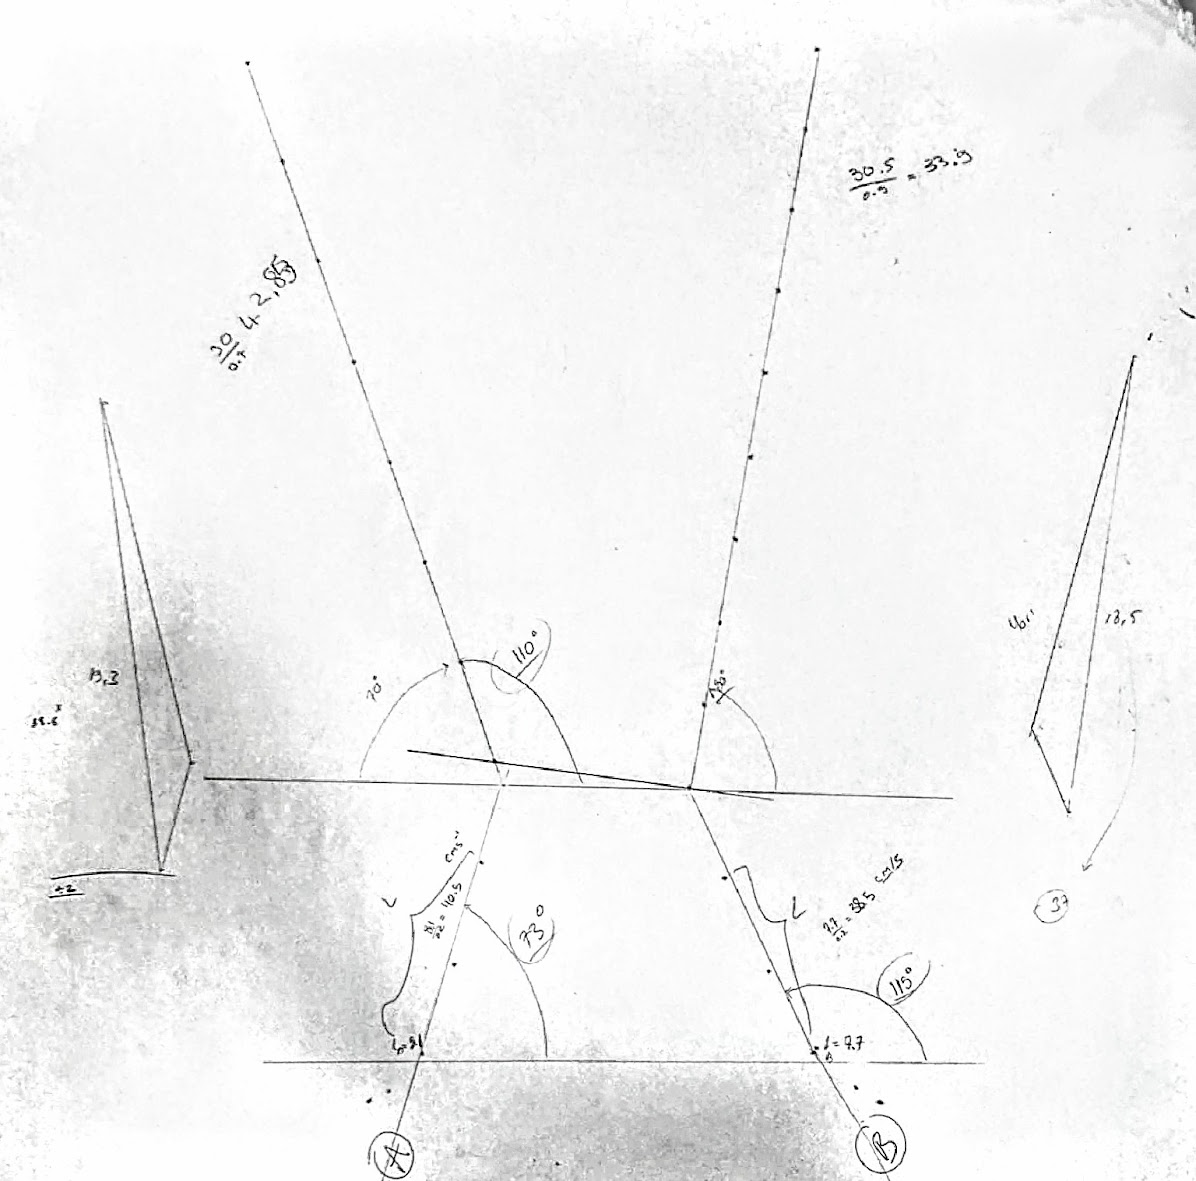
\includegraphics[width=\linewidth]{trajectory.jpg}
    \caption{The recording paper after measurements.}
    \label{fig:traj}
\end{figure}

Table~\ref{tab:Velocity} presents the calculated velocity using the plotted trajectory points, the velocities are then used to derive Table ~\ref{tab:Befor_After} presenting the systems' momentum and kinetic energy before and after the collision by running eq~\ref{eq:ptotal} and ~\ref{eq:ktotal}.
\begin{table}[h]
  \centering
  \begin{tabular}{cccc}
    \hline
    Disc & $v$ ($m/s$) & $v'$ ($m/s$) \\
    \hline
    A & 0.405 & 0.429  \\
    B & 0.385 & 0.339  \\
    \hline \\
  \end{tabular}
  \caption{Veloctiy Before ($v$) and After ($v'$) Collision}
  \label{tab:Velocity}
\end{table}

\begin{table}[h]
    \centering
    \begin{tabular}{ccc}
        \hline
        Property  & $p$ ($kg m/s$)& $K$ ($kg {m^2}/{s^2})$\\
        \hline
        Before collision & 0.391 & 0.083 \\
        After collision & 0.393 & 0.079 \\
        \hline \\
    \end{tabular}
    \caption{Total Momentum ($p$) and Kinetic Energy ($K$), Before and After Collision }
    \label{tab:Befor_After}
\end{table}

From Table~\ref{tab:Befor_After}, relative energy loss is calculated as -0.043 using eq~\ref{eq:relative_energy_loss} \cite{colabnotebook}:
\begin{equation}
    \frac{\Delta E }{E} = \frac{E'- E}{E}
    \label{eq:relative_energy_loss}
\end{equation}
where E and E', are the systems' energy before and after the collision respectively.


\section{Discussion}
The experiment aimed to investigate the conservation of momentum and kinetic energy during the elastic collision of two discs with equal mass. The results reveal important insights into the dynamics of the collision and its conformity to theoretical expectations.

First, let's consider the conservation of momentum. According to the law of conservation of momentum, the total momentum of the system before the collision should be equal to the total momentum after the collision. Mathematically, this is expressed as in eq~\ref{eq:momentum_con}.

From Table~\ref{tab:Befor_After}, we observe that the total momentum before the collision is $0.391 \, \text{kg m/s}$ and after the collision is $0.393 \, \text{kg m/s}$. Although there is a slight increase in momentum after the collision, this can be attributed to experimental errors and the precision of the measurements. Overall, the results confirm the conservation of momentum in the elastic collision.

Next, let's consider the conservation of kinetic energy. The law of conservation of kinetic energy states that the total kinetic energy of the system before the collision should be equal to the total kinetic energy after the collision. Mathematically, this is expressed as in eq~\ref{eq:energy_con}.

From Table~\ref{tab:Befor_After}, we observe that the total kinetic energy before the collision is $0.083 \, \text{kg m}^2/\text{s}^2$ and after the collision is $0.079 \, \text{kg m}^2/\text{s}^2$. This decrease in kinetic energy after the collision is expected in an elastic collision, as some of the kinetic energy is converted into other forms of energy, such as sound or heat, due to imperfections in the collision process. Despite this energy loss, the conservation of kinetic energy is upheld within the experimental limitations.

Finally, comparing the momentum vector analysis (\cite{googledrive}, ATTACHMENT 02), a decent agreement is observed with our results, as we find the total momentum to be approximately 0.390 kg m/s both before and after the collision.

The author recommends reviewing the supplementary materials used in this report in section ~\ref{sec:ad_res}. 
\section{Conclusion}

In this experiment, the conservation of momentum and kinetic energy during the elastic collision of two discs with equal mass was investigated. The velocities and angles of motion were measured from the trajectory paper and reconstructed on millimetric paper to calculate in vector form and verify the results. The total momentum and kinetic energy before and after the collision were analyzed, showing a high degree of agreement. Minor deviations from theoretical expectations can be attributed to experimental errors and environmental factors. Overall, the experiment provides valuable insights into the fundamental principles of physics governing elastic collisions. Future experiments could focus on minimizing these errors to further refine our understanding of elastic collisions.

\section{Additional Resources}
\label{sec:ad_res}
The following resources were used in conducting the experiment:
\begin{thebibliography}{9}
  
  \bibitem{colabnotebook} 
  Google Colab Notebook: Detailed notebook containing extra analysis, and calculations for this experiment (Fig.~\ref{qr:QR}):
  \begin{figure}[h]
      \centering
      
\includegraphics[width=0.25\textwidth]{QR.png}
      \caption{Colab Notebook Link QR, \url{https://colab.research.google.com/drive/1bmyqmDGYYst88uy9dUxbYvYwoU8Lr9r1?usp=sharing}}
      \label{qr:QR}
  \end{figure}

  \bibitem{googledrive}
  Google Drive folder of ATTACHMENT 01 and 02 and Original Recording Paper:
  \begin{figure}[h]
      \centering
      
\includegraphics[width=0.25\textwidth]{Drive.png}
      \caption{G.Drive Folder Link, \url{https://drive.google.com/drive/folders/1z9gcgWBduamGsLnRrat_uz-c6cz2lrz5?usp=drive_link}}
      \label{qr:drive}
  \end{figure}

  \bibitem{textbook} 
  Physics Laboratory textbook: "FİZİK LABROATUVARI DENEY KİTAPÇIĞI [MEKANİK VE SIVILAR]" - İSTANBUL ÜNİVERSİTESİ FEN FAKÜLTESİ FİZİK BÖLÜMÜ.

\end{thebibliography}

\end{document}
